\section*{Question 5}
\fakesection{5}

For this question, we design a Blackman-windowed differentiator filter with 25 taps to the following specifications:
\begin{multicols}{2}
    \begin{itemize}
        \item Sampling frequency: $f_s=50$ kHz
        \item Operating frequencies: 0 Hz to 20 kHz
    \end{itemize}
\end{multicols}
We use the \texttt{scipy.signal.remez} function, specifying the filter type as a `differentiator':
\begin{center}
    taps = \texttt{remez(25, [0, 20], [1], type=`differentiator', fs=50)}
\end{center}
This produces the 25-point discrete impulse response presented in Figure \ref{fig:q5_diff_impz}.

\begin{figure}[ht]
    \centering
    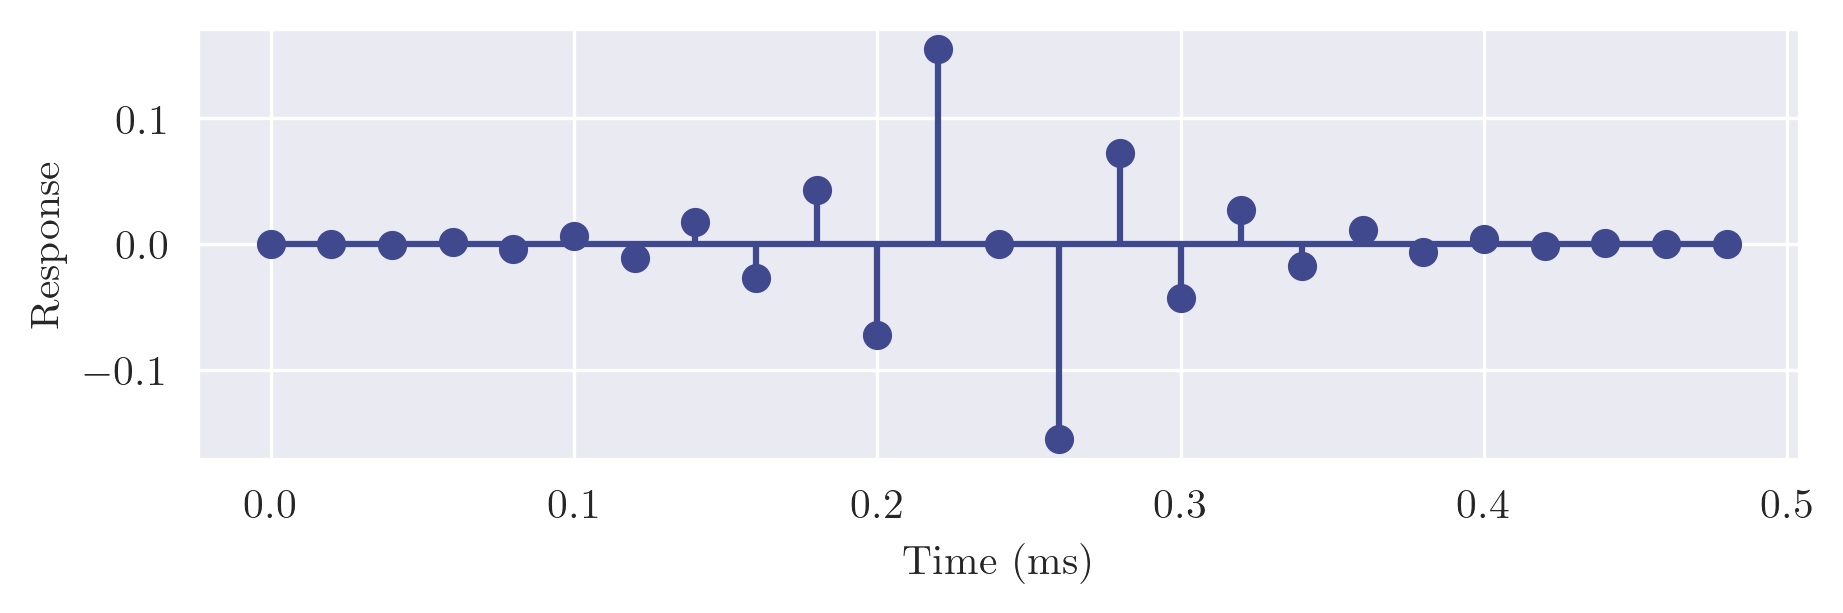
\includegraphics[width=0.8\textwidth]{images/q5_diff_impz.png}
    \caption{Impulse response of differentiator filter}
    \label{fig:q5_diff_impz}
\end{figure}

Applying a Blackman window to the impulse response, we get the following frequency response.

\begin{figure}[ht]
    \centering
    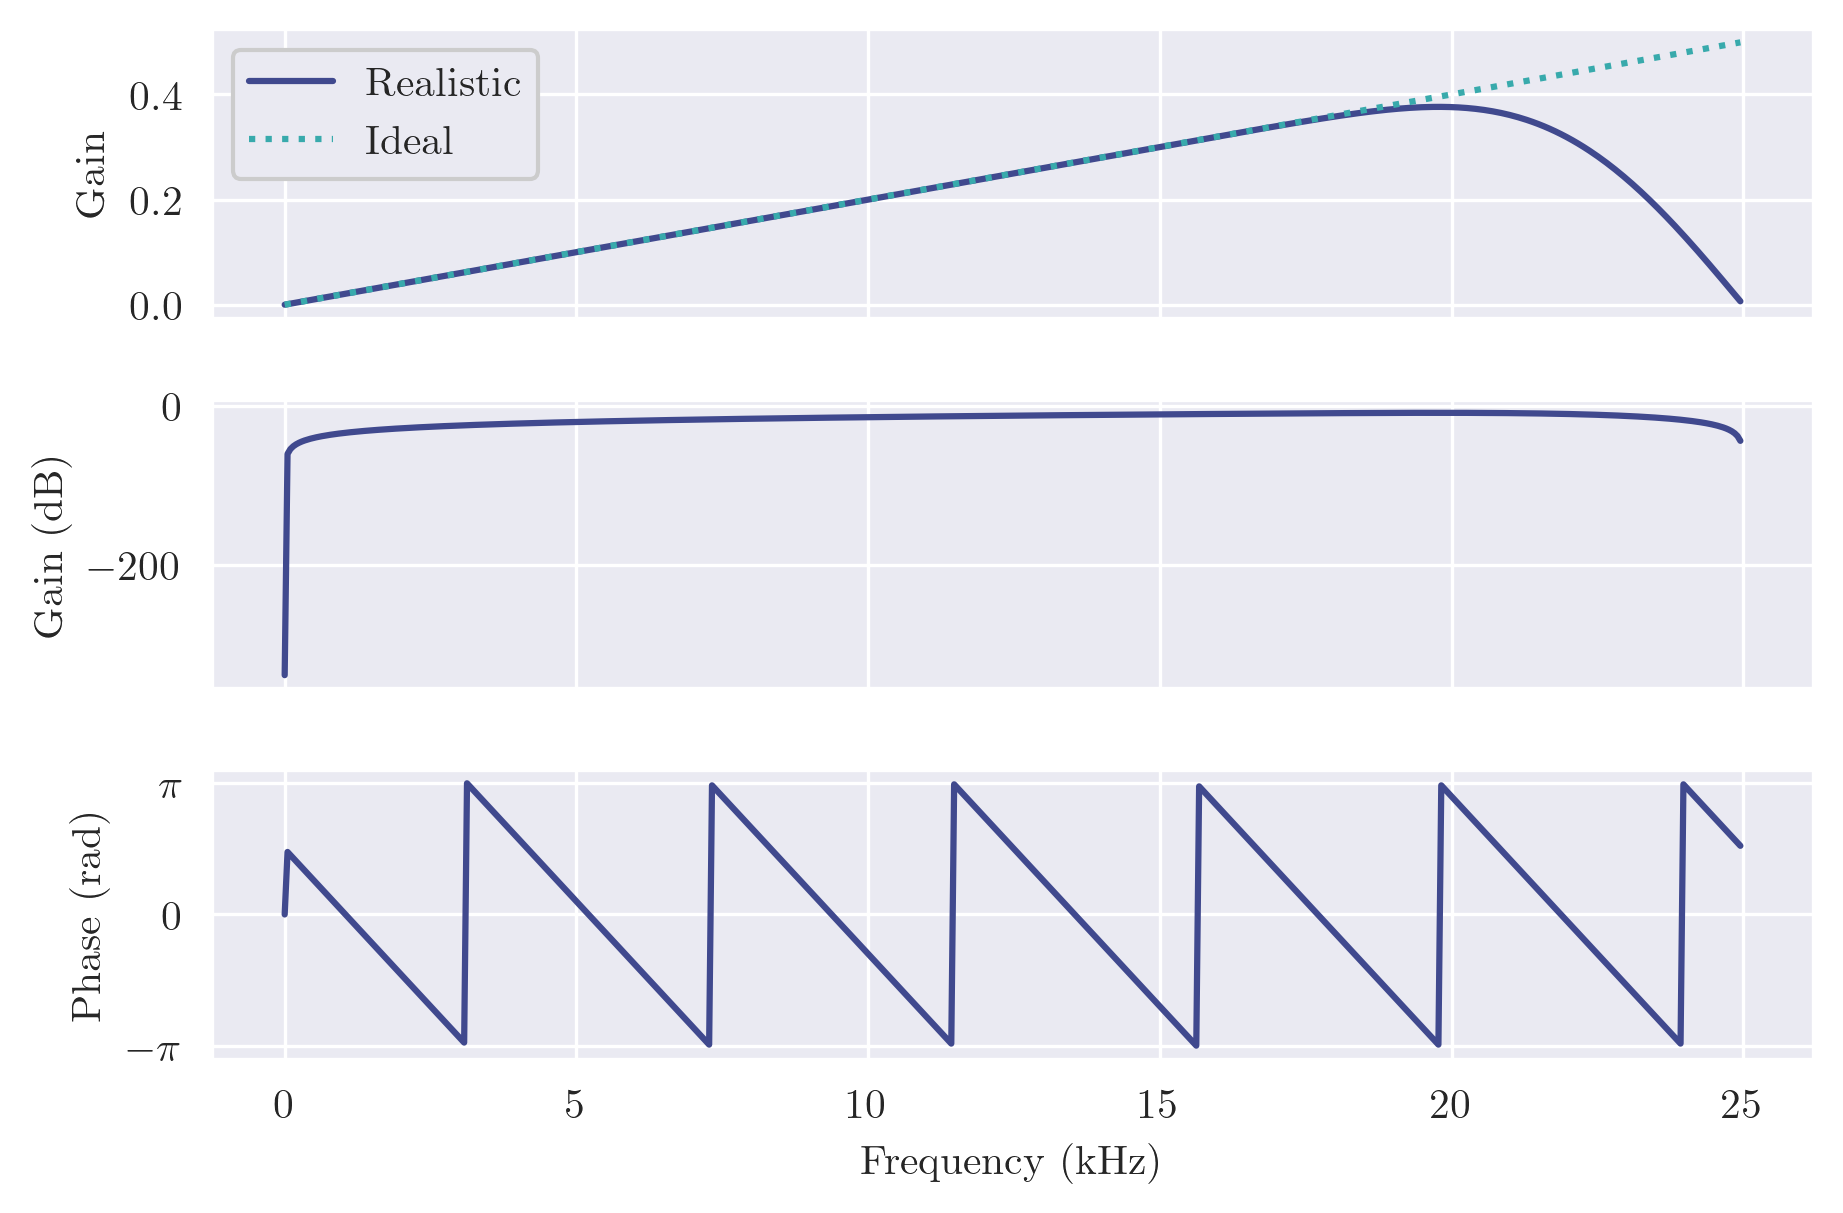
\includegraphics[width=0.8\textwidth]{images/q5_diff_freqz.png}
    \caption{Magnitude and phase frequency response of Blackman-windowed differentiator}
    \label{fig:q5_diff_freqz}
\end{figure}

The filter demonstrates the expected frequency characteristics of an ideal differentiator within its operating range of 0 to 20 kHz; specifically, gain proportional to frequency, and linear phase. The magnitude of slope of the phase is proportional to the length of the filter. A longer filter produces a better approximation of the gain of the ideal differentiator; however, as we will shortly observe, also increases the group delay of the differentiated signal.

\newpage

We now apply the differentiator to various 5 kHz sample signals and observe its effects.

\begin{figure}[!ht]
    \centering
    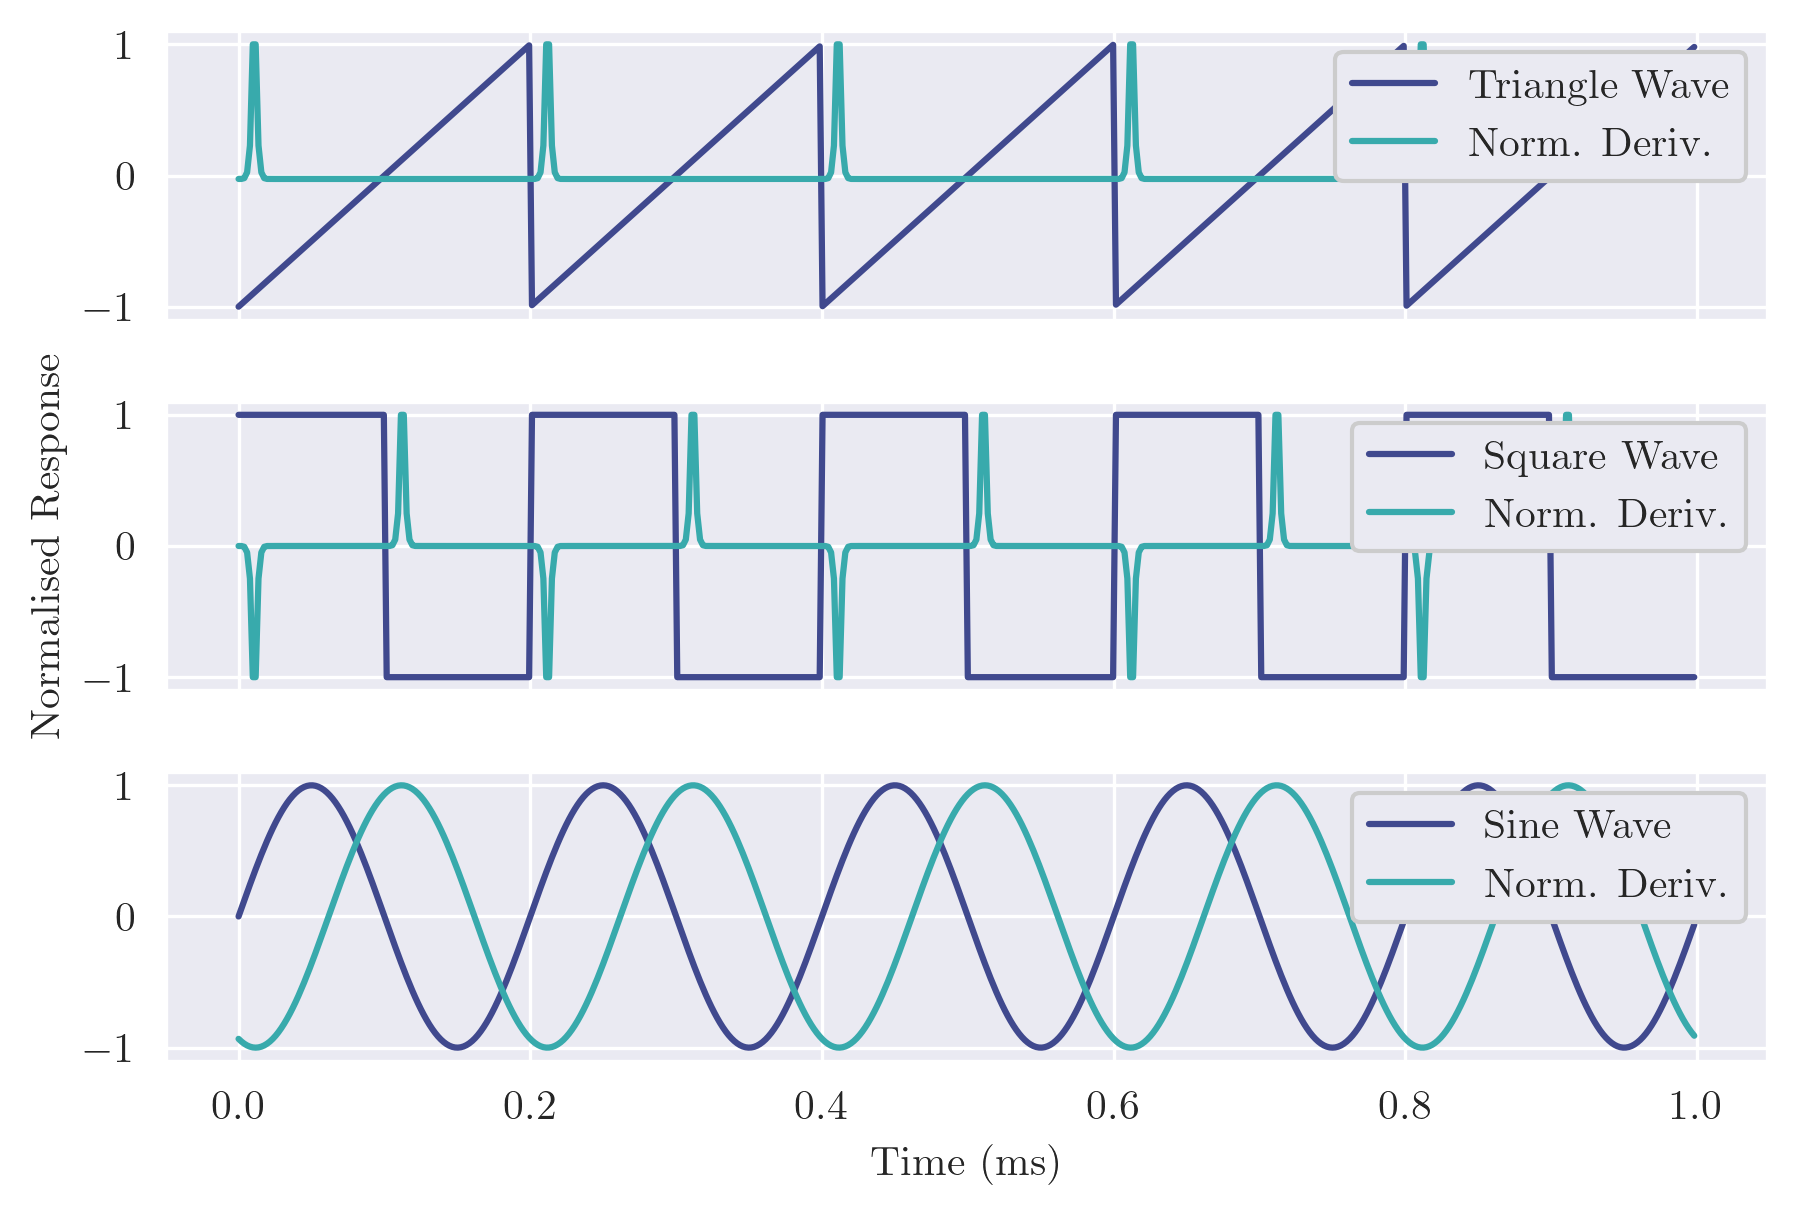
\includegraphics[width=0.8\textwidth]{images/q5_diff_applied.png}
    \caption{Effects of differentiator filter on three sample signals}
    \label{fig:q5_diff_applied}
\end{figure}

The differentiated signal lags the original signal by the group delay, equal to $(N-1)/2$ samples, where $N$ is the filter length\footnote{Q. Chaudhari. ``Design of a Discrete-Time Differentiator.'' WirelessPi.com. https://wirelesspi.com/design-of-a-discrete-time-differentiator/ (accessed Sep. 12, 2023).}. This is also equal to the negative derivative of the filter phase\footnote{A. V. Oppenheim, A. S. Willsky, and H. Nawab, \textit{Signals and Systems}. Upper Saddle River, NJ, USA: Prentice Hall (1997).}.

Intuitively, a (realistic) differentiator is causal and has greatest amplitude around its central coefficients, as is observable in Figure \ref{fig:q5_diff_impz}. This means the full magnitude of the derivative only occurs after passing through half the filter. Of course, because a differentiator is odd length and anti-symmetric, its central coefficient must be zero. Hence, the group delay is $(N-1)/2$.

More rigorously, consider a differentiator in the frequency domain: $H(\omega)=|H(\omega)|e^{-j\omega\alpha}$. The constant $\alpha$ is the gradient of the linear phase. Suppose we apply this filter to the Fourier transform of an input signal, $X(\omega)$, to obtain an output, $Y(\omega)$:
\begin{align}
    Y(\omega) = H(\omega)X(\omega)
              = |H(\omega)|X(\omega)e^{-j\omega n \alpha / N}
\end{align}
In the operating frequency range of the differentiator, $|H(\omega)|\approx 1$; hence,
\begin{align}
    Y(\omega) \approx X(\omega)e^{-j\omega n \alpha / N}
\end{align}
From a basic property of the Fourier transform, we have that
\begin{align}
    y[n] = x[n - \alpha]
\end{align}
Hence, the output is delayed by a constant equal to the negative of the slope of the phase.
